\documentclass[11pt,a4paper]{article}
\usepackage[utf8]{inputenc}
\usepackage{amsmath,amsfonts,amssymb}
\usepackage{graphicx}
\usepackage{geometry}
\geometry{margin=1in}
\usepackage{booktabs}
\usepackage{hyperref}
\usepackage{float}
\usepackage{xcolor}

\definecolor{darkbg}{HTML}{0d121f}
\definecolor{lighttext}{HTML}{e2e8f0}
\definecolor{primary}{HTML}{8b5cf6}
\definecolor{secondary}{HTML}{0dd5c5}
\definecolor{accent}{HTML}{10b981}

\pagecolor{darkbg}
\color{lighttext}

\hypersetup{
    colorlinks=true,
    linkcolor=secondary,
    urlcolor=secondary,
    citecolor=accent
}

\title{\textbf{EE3621: Digital Signal Processing} \\ \Large Student Lecture Notes — Lecture 26 \\ \large Equalization, Noise Cancellation \& Adaptive FIR Filters}
\author{III B.Tech EEE — Core Exam Preparation Guide}
\date{}

\begin{document}

\maketitle

\noindent\rule{\textwidth}{0.5pt}

\section{Channel Equalization \& The Zero-Forcing Equalizer}

\subsection{Inter-Symbol Interference (ISI)}
When digital symbols $s[n]$ are transmitted across a dispersive communication channel $h_c[n]$, multipath delays spread out adjacent symbols, creating **Inter-Symbol Interference (ISI)**:
\begin{equation}
x[n] = s[n] \circledast h_c[n] + v[n] = h_c[0]s[n] + \sum_{k \ne 0} h_c[k]s[n-k] + v[n]
\end{equation}

\subsection{The Zero-Forcing Equalizer (ZFE) Criterion}
An equalizing filter $h_{\text{eq}}[n]$ inverts channel distortion so that the combined response is a pure delay of $\Delta$ samples:
\begin{equation}
H_{\text{eq}}(z) \cdot H_c(z) = z^{-\Delta} \iff \mathbf{q[n] = h_c[n] \circledast h_{\text{eq}}[n] = \begin{cases} 1, & n = \Delta \\ 0, & n \ne \Delta \end{cases}}
\end{equation}
For an $N$-tap FIR equalizer $h_{\text{eq}}[n] = [w_0, w_1, \dots, w_{N-1}]^T$, we force $q[n] = 0$ for $n \ne \Delta$ and $q[\Delta] = 1$, setting up a system of linear algebraic equations to solve for weights $w_k$.

\begin{figure}[H]
\centering
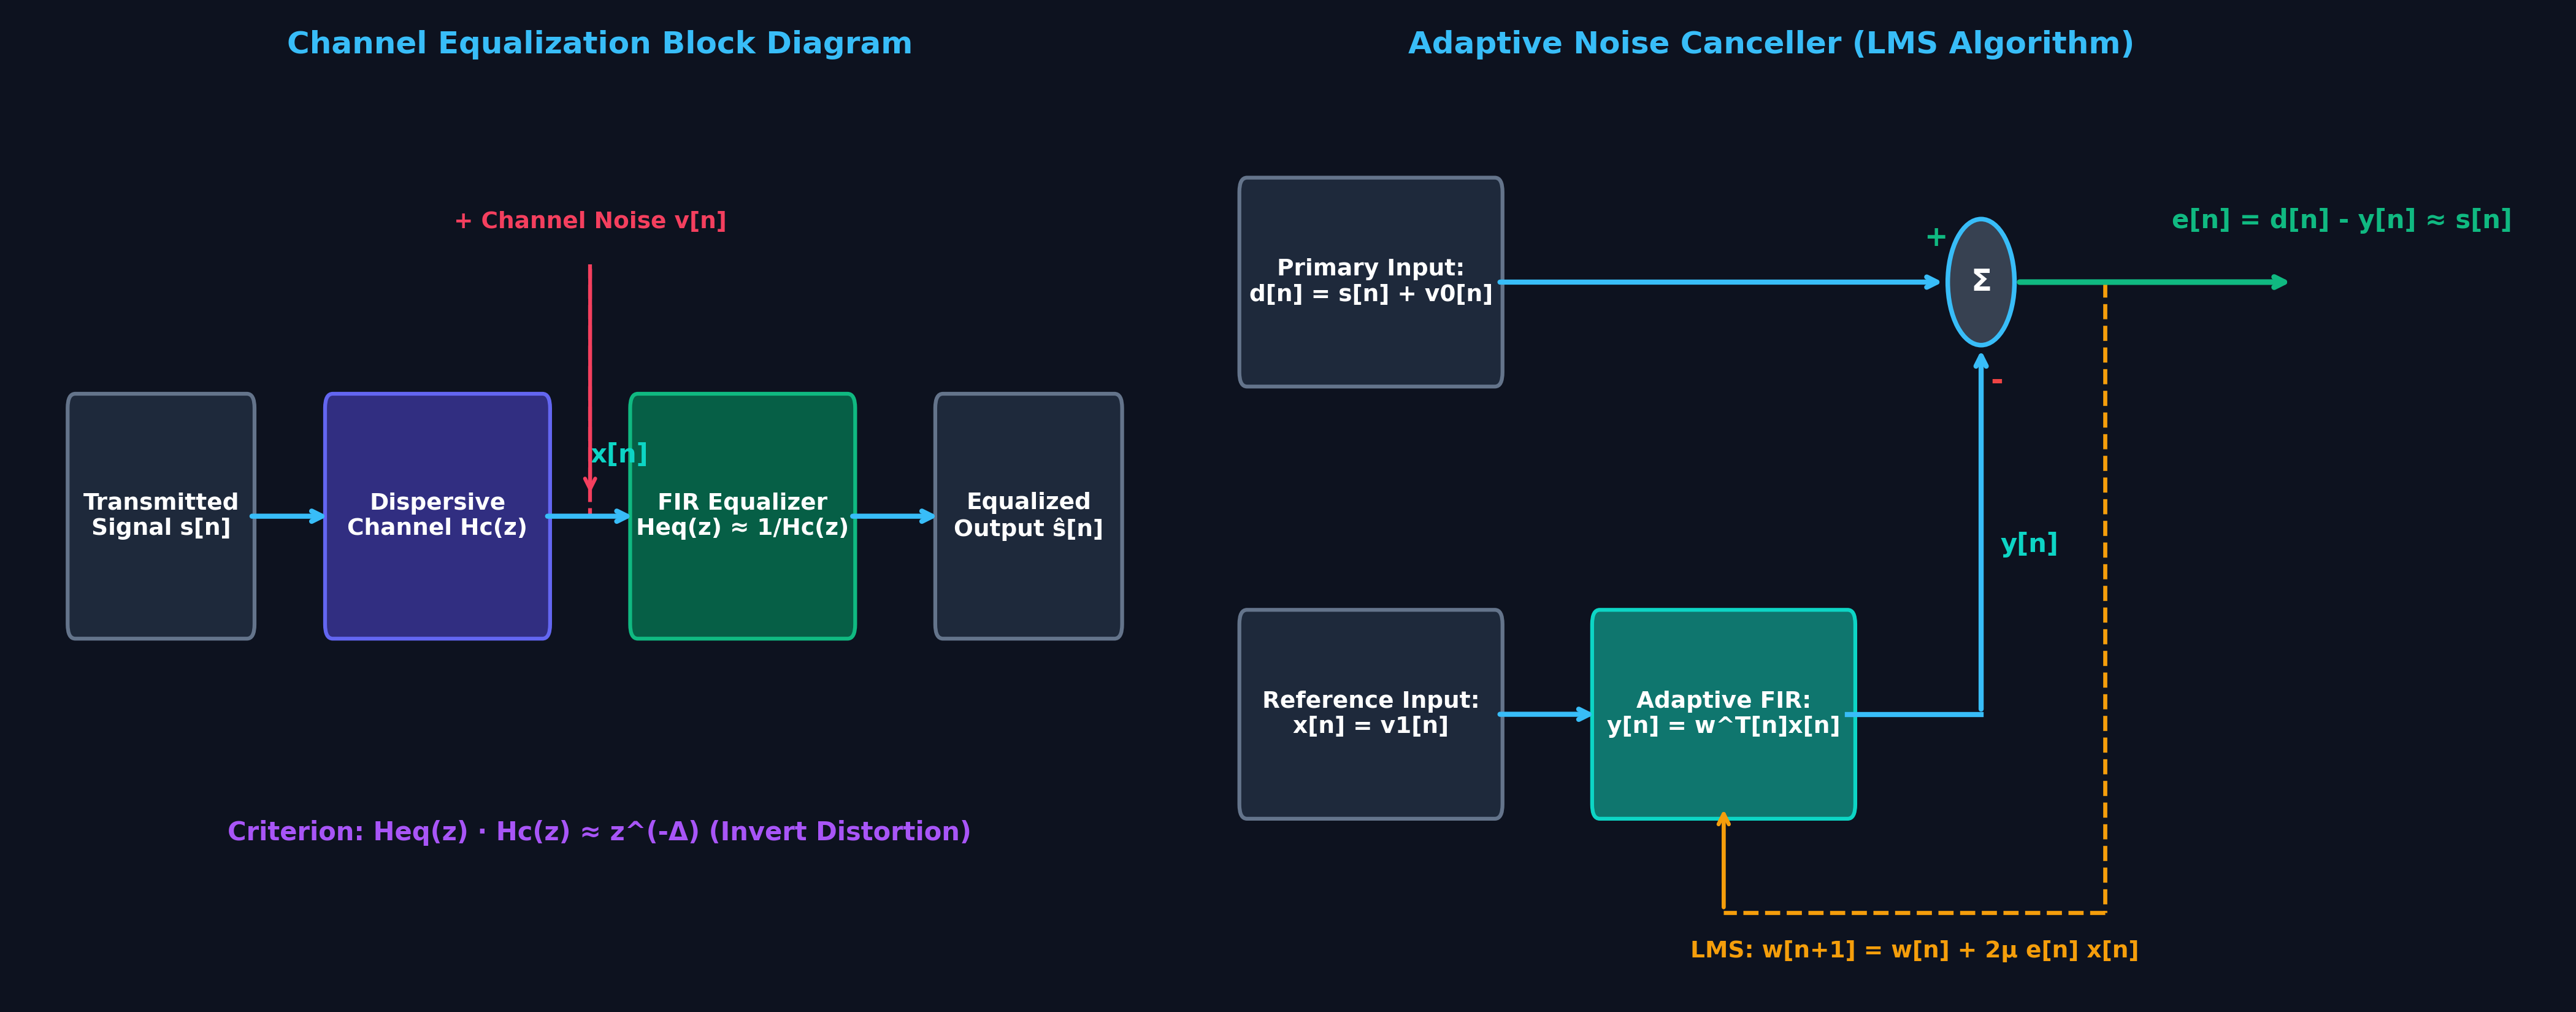
\includegraphics[width=0.88\textwidth]{images/dsp_equalization_noise_cancellation_lms.png}
\caption{Left: Channel Equalizer inverting dispersive channel $H_c(z)$. Right: Dual-input Adaptive Noise Canceller driven by the LMS algorithm.}
\label{fig:dsp_apps_student}
\end{figure}

\noindent\rule{\textwidth}{0.5pt}

\section{Adaptive Noise Cancellation (ANC)}

\subsection{Dual-Input Architecture}
Unlike conventional static filtering, Adaptive Noise Cancellation uses two separate inputs:
\begin{itemize}
    \item \textbf{Primary Input $d[n]$:} Desired signal $s[n]$ contaminated by noise $v_0[n]$:
    \begin{equation}
    d[n] = s[n] + v_0[n]
    \end{equation}
    \item \textbf{Reference Input $x[n]$:} Noise $v_1[n]$ that is correlated with $v_0[n]$, but \textbf{completely uncorrelated with the signal $s[n]$} ($E[s[n] \cdot v_1[n-k]] = 0$).
\end{itemize}

\subsection{Mathematical Proof of Signal Extraction}
The system error output is the difference between primary input and filter estimate $y[n]$:
\begin{equation}
e[n] = d[n] - y[n] = s[n] + \big(v_0[n] - y[n]\big)
\end{equation}
Squaring and taking the statistical expectation:
\begin{equation}
E[e^2[n]] = E[s^2[n]] + E\big[(v_0[n] - y[n])^2\big] + 2 E\big[s[n](v_0[n] - y[n])\big]
\end{equation}
Since $s[n]$ is uncorrelated with both $v_0[n]$ and $y[n]$, the cross-term is zero:
\begin{equation}
\mathbf{E[e^2[n]] = E[s^2[n]] + E\big[(v_0[n] - y[n])^2\big]}
\end{equation}
\textbf{The Core Principle:} Signal power $E[s^2[n]]$ is unaffected as filter weights adapt. Therefore, minimizing total output power $E[e^2[n]]$ forces:
\begin{equation}
y[n] \longrightarrow v_0[n] \implies \mathbf{e[n] \longrightarrow s[n]}
\end{equation}
The system error output $e[n]$ becomes the **clean, noise-free signal**!

\noindent\rule{\textwidth}{0.5pt}

\section{The Adaptive FIR Filter \& The LMS Algorithm}

\subsection{The 3 Core Operational Equations of LMS}
For an $M$-tap adaptive transversal FIR filter with weight vector $\mathbf{w}[n] = [w_0[n], \dots, w_{M-1}[n]]^T$ and input vector $\mathbf{x}[n] = [x[n], \dots, x[n-M+1]]^T$:
\begin{enumerate}
    \item \textbf{Filter Output:}
    \begin{equation}
    \mathbf{y[n] = \mathbf{w}^T[n] \mathbf{x}[n] = \sum_{k=0}^{M-1} w_k[n] x[n-k]}
    \end{equation}
    \item \textbf{Error Estimation:}
    \begin{equation}
    \mathbf{e[n] = d[n] - y[n]}
    \end{equation}
    \item \textbf{Widrow--Hoff Weight Update:}
    \begin{equation}
    \mathbf{\mathbf{w}[n+1] = \mathbf{w}[n] + 2\mu \, e[n] \, \mathbf{x}[n]}
    \end{equation}
    or for each individual tap: $\mathbf{w_k[n+1] = w_k[n] + 2\mu \, e[n] \, x[n-k]}$.
\end{enumerate}

\subsection{Step-Size Parameter \texorpdfstring{$\mu$}{mu} Stability Criterion}
To guarantee convergence without divergent numerical instability:
\begin{equation}
\mathbf{0 < \mu < \frac{1}{M \cdot P_x}}
\end{equation}
where $M$ is the number of filter taps and $P_x = E[x^2[n]]$ is the input signal power.

\noindent\rule{\textwidth}{0.5pt}

\section{Standard Solved Exam Example}

\textbf{Problem:} A 2-tap adaptive FIR filter has initial weights $\mathbf{w}[0] = [0.0, \; 0.0]^T$ and adaptation step-size $\mu = 0.1$. Given the input sequences:
\begin{itemize}
    \item At $n = 0$: Reference vector $\mathbf{x}[0] = [1.0, \; 0.5]^T$, Primary target $d[0] = 2.0$.
    \item At $n = 1$: Reference vector $\mathbf{x}[1] = [0.5, \; 1.0]^T$, Primary target $d[1] = 1.5$.
\end{itemize}
Compute the filter output $y[n]$, error $e[n]$, and updated weight vector $\mathbf{w}[n+1]$ for iterations $n = 0$ and $n = 1$.

\vspace{1mm}
\noindent\textbf{Solution:}

\noindent\textbf{Iteration 1 ($n = 0$):}
\begin{enumerate}
    \item \textbf{Filter Output $y[0]$:}
    \begin{equation}
    y[0] = w_0[0]x[0] + w_1[0]x[-1] = (0.0)(1.0) + (0.0)(0.5) = \mathbf{0.0}
    \end{equation}
    \item \textbf{Error $e[0]$:}
    \begin{equation}
    e[0] = d[0] - y[0] = 2.0 - 0.0 = \mathbf{2.0}
    \end{equation}
    \item \textbf{Weight Vector Update $\mathbf{w}[1]$:}
    With $2\mu = 2(0.1) = 0.2$:
    \begin{equation}
    2\mu e[0] = 0.2 \times 2.0 = 0.4
    \end{equation}
    \begin{equation}
    w_0[1] = w_0[0] + 0.4 x[0] = 0.0 + 0.4(1.0) = \mathbf{0.40}
    \end{equation}
    \begin{equation}
    w_1[1] = w_1[0] + 0.4 x[-1] = 0.0 + 0.4(0.5) = \mathbf{0.20}
    \end{equation}
    Updated weight vector: $\mathbf{w}[1] = [0.40, \; 0.20]^T$.
\end{enumerate}

\noindent\textbf{Iteration 2 ($n = 1$):}
\begin{enumerate}
    \item \textbf{Filter Output $y[1]$:}
    \begin{equation}
    y[1] = w_0[1]x[1] + w_1[1]x[0] = (0.40)(0.5) + (0.20)(1.0) = 0.20 + 0.20 = \mathbf{0.40}
    \end{equation}
    \item \textbf{Error $e[1]$:}
    \begin{equation}
    e[1] = d[1] - y[1] = 1.5 - 0.40 = \mathbf{1.10} \quad \text{(Error reduced from 2.0 to 1.10!)}
    \end{equation}
    \item \textbf{Weight Vector Update $\mathbf{w}[2]$:}
    \begin{equation}
    2\mu e[1] = 0.2 \times 1.10 = 0.22
    \end{equation}
    \begin{equation}
    w_0[2] = w_0[1] + 0.22 x[1] = 0.40 + 0.22(0.5) = 0.40 + 0.11 = \mathbf{0.51}
    \end{equation}
    \begin{equation}
    w_1[2] = w_1[1] + 0.22 x[0] = 0.20 + 0.22(1.0) = 0.20 + 0.22 = \mathbf{0.42}
    \end{equation}
    Final weight vector: $\mathbf{w}[2] = [0.51, \; 0.42]^T$.
\end{enumerate}

\noindent\rule{\textwidth}{0.5pt}

\section{Essential Exam Checklist \& Traps}
\begin{itemize}
    \item[$\square$] \textbf{LMS Order of Operations:} Always compute in strict order: $y[n] \to e[n] \to \mathbf{w}[n+1]$. Never update weights before computing the output!
    \item[$\square$] \textbf{The Factor of 2 in LMS:} Remember the update is $\mathbf{w}[n+1] = \mathbf{w}[n] + 2\mu e[n]\mathbf{x}[n]$.
    \item[$\square$] \textbf{Reference Input Isolation:} In ANC, the reference input $x[n]$ must contain **only noise**; it must never contain the desired signal $s[n]$.
    \item[$\square$] \textbf{Step-Size Bounds:} Selecting $\mu > 1/(M P_x)$ leads to immediate mathematical divergence ($w_k \to \infty$).
\end{itemize}

\end{document}
